% this file is called up by thesis.tex
% content in this file will be fed into the main document

%: ----------------------- name of chapter  -------------------------
\chapter{Literature review} \label{ch3} % top level followed by section,  subsection

In this Chapter, we provide a taxonomy of the existing outcome-oriented PPM methods for business manners, including a systematic overview of current techniques for encoding and evaluating these methods. In recent years the area of PPM becomes very rich and has many different ways and evaluation methods, so we decided to focus on the outcome-oriented PPM only.

This Chapter will clarify the subsequent research questions:


	\begin{itemize}[itemindent=0em]
		\item[\textbf{RQ1}] What are the existing approaches for building and training a predictive model using a historical labelled data of an event log that contains a set of complete traces with its outcome that can accurately predict incomplete business cases during its execution time?.		
		\item[\textbf{RQ2}]  How to combine these techniques into a taxonomy?		
		\item[\textbf{RQ3}] How to quantify the goodness or badness for these methods?  
			
	\end{itemize}
%\end{framed}

In section, \ref{rq12} we answer and describe RQ1 and RQ2, wherein section \ref{sec32}, we continue with RQ3.  In section \ref{s3}, we conclude this Chapter. 

%: ----------------------- paths to graphics ------------------------

% change according to folder and file names
\ifpdf
    \graphicspath{{X/figures/PNG/}{X/figures/PDF/}{X/figures/}}
\else
    \graphicspath{{X/figures/EPS/}{X/figures/}}
\fi


 

\section{Outcome-oriented PPM methods and Taxonomy} \label{rq12}
In this section, we introduce a taxonomy of the existing outcome-oriented PPM methods for business processes. Our aim from this section is to answer RQ1 (What are the current techniques to train outcome-oriented predictive models) and RQ2 (How to combine these methods). Within the taking after subsections, we begin with presenting the concepts and the work-flow for outcome-oriented PPM, continue with characterizing the existing approaches concerning the diverse steps discernible in the work-flow and conclude with a scientific categorization for the examined methods.


\subsection{Outcome-oriented PPM Basics and work-flow.} \label{wf}
All reviewed methods use universal principles and concepts. We defined some of them in Chapter \ref{ch1} (e.g. event log, trace, etc.)
In outcome-oriented PPM, forecasts are formed using a supervised machine learning method (or classifier) which uses as input data a set of independent attributes $X$ ( or feature vector) and learns a function $f$ that maps $X \to y$ where $y$ is the outcome of the ongoing business case. To feed a classification model with an event log as input, we define \textit{trace encoder} to encode all traces in this log into a feature vector.

\begin{definition}{\textit{\textbf{Trace encoder}}}
	A trace (or sequence) encoder \textit{seq\_enc:} $R_* \to X_1 \times \dots \times X_d$ is a function that takes a business case $\sigma$ and encodes it to a numeric feature vector toward the  $d$-dimensional vector space  $X_1 \times \dots \times X_d$ with $X_k \subseteq \mathbb{R}, 1 \le k \le d $ being the domain in $k$-th independent variable. 	
\end{definition} 

\begin{definition}{\textit{\textbf{Classifier}}}
		A binary classifier \textit{clf}: $X_1 \times \dots \times X_d \to [0, 1]$ is a method $f$ that takes $d$-dimensional feature vectors as input and maps each vector into a target label through a prediction score reflecting the probability of the positive target. 		
\end{definition} 
In predictive process monitoring, we teach a $clf$ how to learn from a historical \textit{prefix log} during the training operation. 

\begin{definition}{\textit{\textbf{Prefix log}}}
	A prefix log $E_* \subset E$  is an event log that includes a subset of prefixes of $E$. The prefix log contains all possible prefixes from an event log.
	Prefixes can be grouped into buckets using a bucketing function and for each bucket, $B$ we train a separate classifier $clf$.		
\end{definition}

\begin{definition}{\textit{\textbf{Bucketing function}}}
	A bucketing function $bucketer: R_* \to \mathbb{N}$ is a method that takes a business case $\sigma$ and put it inside a bucket $b_i$ where $1 \le i \le B$, and $B$ is the total number of all possible buckets. 		
\end{definition}
In this context and taking into account these concepts, we describe a predictive model as follows. 

\begin{definition}{\textit{\textbf{Predictive model}}}
	A predictive model is a general function $Pred: R_* \to [0,1]$ that takes a running case (or trace) $\sigma$ as an input and do three main things based on the above definitions: (\romannumeral 1) assign this trace into a particular bucket $b_i$ based on the bucketing function;  (\romannumeral 2) encode $\sigma$ into a feature vector based on the $seq_enc$ function; (\romannumeral 3) estimate the probability of the positive outcome based on $Pred$ function.  In other words $pred (\sigma) = clf_{bucketer(\sigma)}(seq_{enc}(\sigma))$.	 		
\end{definition}
 
 
The common work-flow for outcome-oriented PPM can be viewed as two main steps \cite{teinemaa2019outcome}. (\romannumeral 1) \textit{Off-line} step to teach (or train) a predictive model on how to learn from historical event logs (see figure \ref{fig:ppmwf}), this step can be decomposed into four steps. First, we extract all possible prefixes from a given event log. Next, Based on the similarities between the extracted prefixes, we separate them into a set of buckets. After that, we encode each bucket into a feature vector to train a separate classifier for each bucket which is the final step. (\romannumeral 2) \textit{On-line} step, where we can predict the final outcome for the running traces using the trained classifiers, and prefix buckets form the off-line step. Particularly, for a running case, we determine the corresponding bucket from historical buckets first, then we encode this running trace into a feature vector using an encoder, and finally based on the selected bucket we chose the corresponding classifier to predict the final outcome of this case.  In the subsequent subsections, we explain the four steps of the off-line step and utilize this description to build a taxonomy about existing methods for outcome-oriented predictive process monitoring. 


\begin{figure}[htb]
	\begin{center}
		\resizebox{10cm}{!}{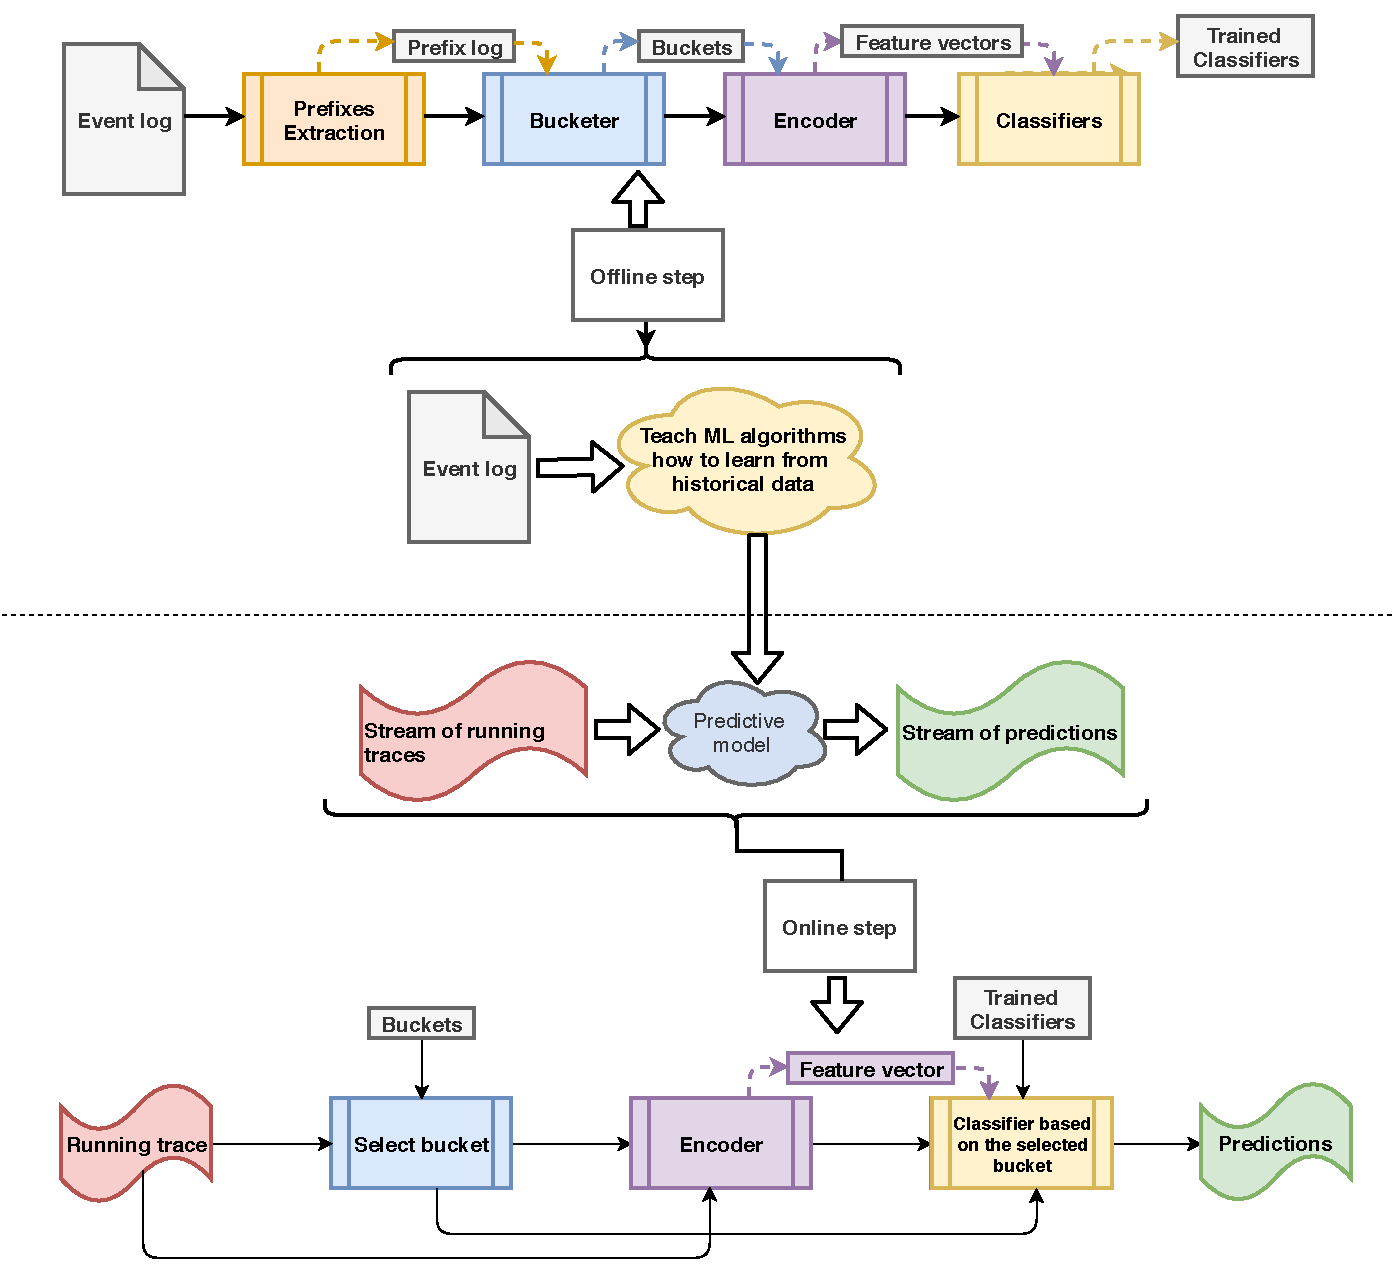
\includegraphics{images/general/ppmwf.pdf}}
		\caption[Detailed Predictive process monitoring workflow]{A detailed predictive process monitoring workflow, including trace bucketing, sequence encoding, and classification for online and offline steps. }
		\label{fig:ppmwf}
	\end{center}
\end{figure}

\subsection{Prefix extraction}
In outcome-oriented PPM, we aim to predict the final outcome of the ongoing business case (running trace), it means the unseen data for our classifier is a prefix log. Because of that, it’s obvious to train this classifier on a prefix log as well to make training and testing operations comparable.  In this context, we define how to extract prefixes from a historical event log. 

In this thesis, we are dealing with 20 different event logs from real-life and extracting all possible prefixes from these logs may raise many problems during the training process for predictive models. (\romannumeral 1) Different length of the business cases in the original event generates different prefixes; in other words,  more prolonged cases generate more prefixes and affect the training process by making classifiers to be biased to them. (\romannumeral 2) The training process with a large number of prefixes is a bottleneck because it will take more and more time and slow down the whole training process.  Thereby, it is standard to extract prefixes from the original event log up to a specific number.  In \cite{leontjeva2016complex}, they extracted prefixes up to $30$ events only, at the same time \cite{verenich2016complex} limits the length of prefixes up to $20$.

\subsection{Trace bucketing}
In outcome-oriented PPM, training multiple classifiers for different buckets is very common. Based on the similarities between prefix traces in the original event log, we can divide them into different buckets, then train a binary classifier for each bucket individually. During the execution time of any ongoing case, we select the most suitable bucket for that case, after that apply the respective classifier on it to predict the outcome of that case.  In this subsection,  we present the bucketing methods that have been introduced by current PPM techniques.

\textbf{\textit{Single bucket}}.  This approach has been introduced in \cite{de2016general}. In this method, all prefix traces are not split into different buckets and considered to be within the same bucket (single bucket). Accordingly, there is no need to train multiple classifiers in these methods, after that we apply the trained classifier to the ongoing cases during their execution time.  

\textbf{\textit{KNN bucketing}}. This method has been introduced in \cite{maggi2014predictive}. This method does not follow the same general workflow we introduced in section \ref{wf} and skip the off-line step, in addition to the prefixes are not split into different buckets.  Alternatively, for any prefix trace and based on the $KNN$ algorithm that selects $K$ nearest neighbours for any training or testing sample, it selects the $k$ nearest neighbours (i.e. based on similarities between traces using string-edit distance) for that trace then puts them into a single bucket and trains a classifier on top of the generated bucket. In this context, the number of buckets and classifiers are not fixed and grow based on incoming events.

\textbf{\textit{Cluster bucketing}}.  This approach was introduced by \cite{di2017clustering}. In this method, the trace prefixes are split into different buckets (or clusters) using various clustering algorithms such as \textit{DBScan}, or \textit{hierarchical clustering}. Accordingly, we train a classifier for each resulting cluster by taking into account prefix traces on each cluster only. During the execution time of the ongoing case, a cluster is selected based on historical clusters; then the relevant classifier is applied. In \cite{di2017clustering}, they used two different clustering algorithms, the first one depends on \textit{string-edit} distance, i.e. \textit{DBScan}, and the other one based on \textit{Euclidean distance}


\textbf{\textit{State bucketing}}. In this approach prefix traces are divided into buckets based on the similarities between trace states, i.e. each component (e.g. task) in the process model is relative to a particular \textit{state}). During the execution time of the ongoing case, a bucket is selected based on historical buckets; then the relevant classifier is applied. This approach depends mainly on having the process model earlier. In the literature, there are predictive methods based on the state approach that a process model and an event log as an input, and they assume that the process model meets the event log accurately such as \cite{grigori2001improving, conforti2015recommendation, schwegmann2013method}. Alternatively, in \cite{lakshmanan2010predictive}, they introduced a method to directly generate a process model of the given event log. 

\textbf{\textit{Prefix length bucketing}}. This method has been introduced in \cite{leontjeva2016complex, van2012process}. The idea of this bucketing method is to build a bucket for each prefix length. For example, the first bucket contains three events from a trace, and the second bucket includes four events from a trace, and so on. For each bucket, one classifier is trained to predict the ongoing cases during their execution time. 

\subsection{Sequence encoding}
To teach a machine learning algorithm how to learn from a historical event log, all prefixes in all buckets need to be \textit{encoded} into a feature vector. This encoding step is a little bit challenging because of the nature of event log attributes. \textit{Event attributes} are \textit{dynamic} and change during all incoming events; therefore, more data regarding the case becomes accessible. On the other hand, \textit{case variables} are \textit{static} for the whole business case. To tackle this problem a trace abstraction technique \cite{van2010process} can be used; after that, we use feature extraction methods to encode prefixes into feature vectors. In this context, many sequence encoding methods have been surveyed in \cite{leontjeva2016complex}, and \cite{teinemaa2019outcome}. In the coming paragraphs, we present different encoding methods that can be used in outcome-oriented PPM problems. 

\textbf{\textit{Static encoding}}.
This method was introduced in \cite{leontjeva2016complex}. Case attributes remain the same within the whole case that makes the encoding process very simple, and we keep it without any loss of information. To exemplify categorical attributes as numeric features \textit{one-hot} encoding or \textit{get dummies} methods can be used. 

\textbf{\textit{Last state}}.
 In this approach, only the very last $m$ event attributes are measured. For this reason, the feature vector size is fixed during the execution of a case and proportional to the number of event attributes. A drawback of this approach is that anything that happened in the past and capture information will be neglected, i.e. information loss. This encoding method is commonly used with the $KNN$ method \cite{maggi2014predictive},  and state-based bucketing \cite{conforti2015recommendation}.

\textbf{\textit{Aggregation}}. In this approach, the drawback in the last state method that is \textit{lossy encoding} is solved by considering all events since the beginning of the business case. Many aggregation functions are used with numerical attributes such as \textit{max, min, average,} and \textit{sum} as well as with categorical attributes such as \textit{count} \cite{de2016general} to make sure the size of the feature vector is constant. Although this method considers all events, it neglects the order of events which is the drawback of this method.

\textbf{\textit{Index-based encoding}}. This method was introduced in \cite{van2012process}. It uses all possible information in the case by considering all events as the aggregation method and also the order of events. The advantage of this method is that it is considered as a \textit{lossless} (i.e. we can construct the original trace from its feature vector) encoding method.  A drawback of this method is it can be used only with homogeneous (i.e. all traces have the same length) buckets. 

All encoding methods are dealing with event attributes except the static method where it deals with case attributes. Figure \ref{fig:enc1} shows a summary of  all encoding methods with trace abstraction. 

\begin{figure}[htb]
	\begin{center}
		\resizebox{10cm}{!}{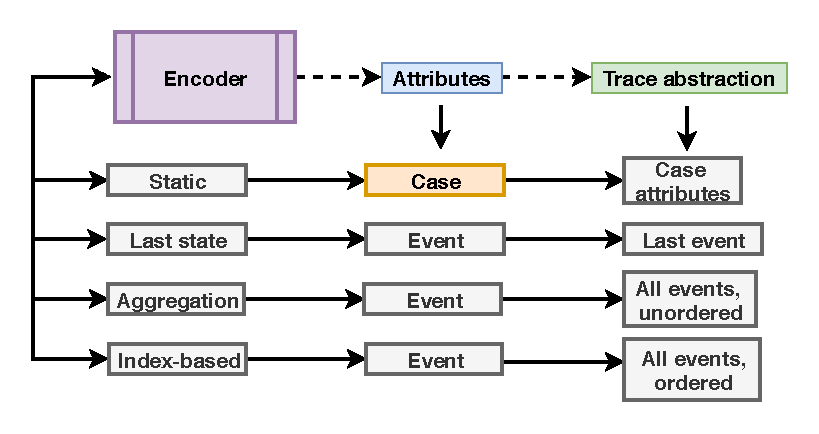
\includegraphics{images/general/enc1.pdf}}
		\caption[Encoding methods and trace abstraction]{Taxonomy of current sequence encoding techniques for PPM such as static, last state, etc., and trace abstraction for each technique.}
		\label{fig:enc1}
	\end{center}
\end{figure}

\subsection{Classification algorithms}
Outcome-oriented PPM task is considered as a classification problem that aims to predict the outcome on ongoing cases during its execution time. Current outcome predictive methods have been examined with many classification algorithms. Decision tree algorithm is The most popular classifier that is used for PPM tasks \cite{de2016general, grigori2001improving, maggi2014predictive}. Also, RF has been used in many studies before, such as \cite{leontjeva2016complex, ghattas2014improving}. Furthermore, SVM \cite{schwegmann2013method}, KNN \cite{van2012process}, and Gradient Boosting methods \cite{teinemaa2019outcome}. 

\subsection{Discussion}
Outcome-oriented PPM is a very growing research area. In this Chapter, we give a complete analysis of existing outcome-oriented PPM methods that aim to predict the outcome of a business case during its execution time. On the basis of the above, we conclude that prefix extraction methods are  not characteristic to any given PPM techniques. Alternatively, these methods are chosen on the basis of the performance measure and can be utilized by all PPM techniques. In the same context, machine learning algorithms are growing very fast, and there is no rule of thumb to use a particular algorithm with particular business process data, and again the performance metric is the judge to choose between different algorithms. 
To categorize current outcome-oriented PPM, we should identify two main things: (\romannumeral 1) How to split prefix traces into several buckets; (\romannumeral 2) How to encode each prefix in each bucket into a feature vector.  To answer those two questions, we provide a taxonomy (see figure \ref{fig:bucenc}) of the appropriate methods based on those two viewpoints plus different classification algorithms that have been used for outcome-oriented PPM. 

\begin{figure}[htb]
	\begin{center}
		\resizebox{10cm}{!}{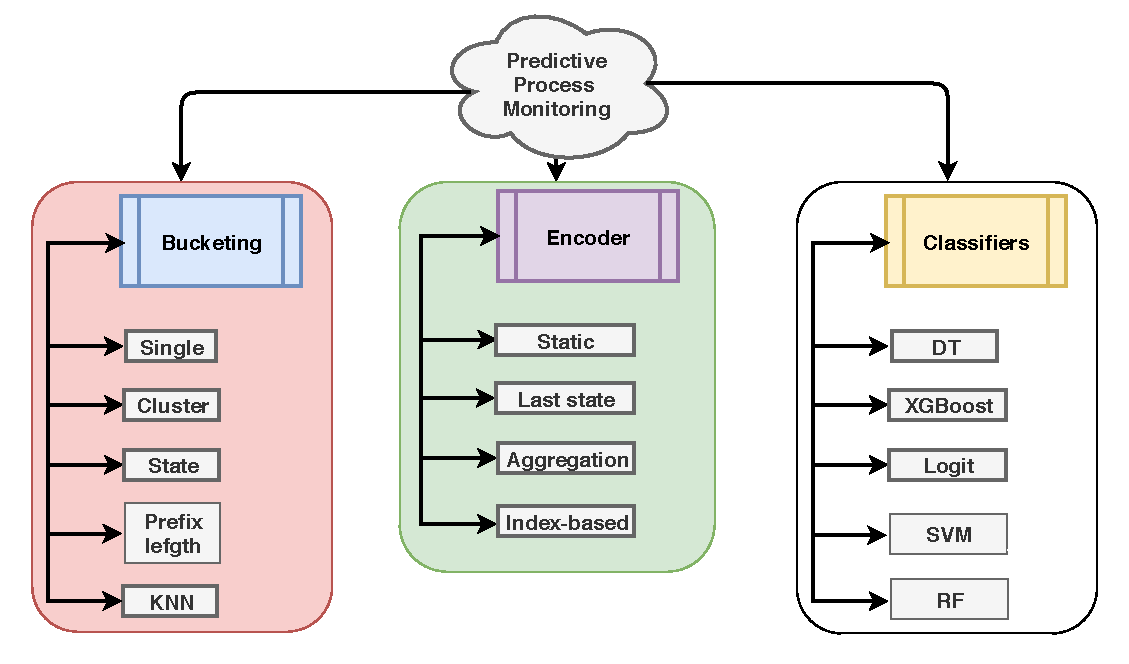
\includegraphics{images/general/tax.pdf}}
		\caption[Taxonomy of methods for outcome-oriented PPM]{Taxonomy of existing sequence encoding, trace bucketing, and classification methods for outcome-oriented PPM.}
		\label{fig:bucenc}
	\end{center}
\end{figure}



\section{Evaluation measures and experimental settings} \label{sec32}
To quantify the goodness or badness of an outcome-oriented PPM, different evaluation measures can be used. In this section, we provide possible evaluation measures in the literature. In outcome-oriented PPM a right prediction ought to be correct (or accurate) and it ought to be executed in the beginning steps of the operation as well as it should be produced efficiently. In the following passages, we dive into these measures.


\textbf{\textit{Accuracy.}} It refers to the relation between the correctly classified cases compared to the actual true labels, i.e. ground truth and all classified cases. Inaccurate predictions are useless as it does not help with making decisions. Accordingly, accuracy is considered as the most important measure of a prediction. 
Classification models give output as a real-valued score to estimate how likely this case belongs to a positive or negative class or binary values that reflect a positive or negative class. In binary values outcome, it is common to use metrics that we can derive from the confusion matrix (see Chapter 2), e.g. accuracy, precision, recall, and F-score. In real-valued outcome, the most commonly used metric is AUC, i.e. area under the curve. In continuous predictive monitoring (i.e. the system worker gets predictions about the ongoing cases after each event where the system doesn't tell the worker how to intervene to avoid undesired outcome) prediction accuracy is mostly stated at different prefix lengths or evaluation points \cite{verenich2016complex, van2012process, leontjeva2016complex}. Furthermore, the net accuracy is calculated as the average of accuracy through all evaluation points.

\textbf{\textit{Earliness}}. In predictive process monitoring, it is imperative to predict the final outcome as soon as possible to give the process worker the ability to act against unexpected outcomes. In continuous predictive monitoring, earliness is measured at different evaluation points implicitly or explicitly \cite{leontjeva2016complex}. 


\textbf{\textit{Efficiency}}. In PPM systems, it is important to predict the outcome in an acceptable time. Accordingly, Execution time taken during online and offline steps are computed to report the efficiency of a model. In \cite{di2017clustering}, they split the execution time taken during the online step into \textit{processing time}, i.e. time was taken to encode and assign test prefixes into buckets and \textit{prediction time}, i.e. the average time to predict the outcome for a given prefix.  


%Summary of each chapter is MANDATORY
\section{Summary} \label{s3}
In this Chapter, we answered \textit{RQ1}, \textit{RQ2}, and \textit{RQ3}, and at the same time, we give a comprehensive review of the current outcome-oriented predictive process monitoring. In the next Chapter, we start by introducing the methods we propose in this thesis to improve the outcome-oriented predictive process monitoring techniques. 





% ---------------------------------------------------------------------------
%: ----------------------- end of thesis sub-document ------------------------
% ---------------------------------------------------------------------------

